%\documentclass{article}
%
%%\usepackage[pdf]{pstricks}
%\usepackage{hyperref}
%\usepackage{pdfpages}
%
%\title{Project Proposal and Plan}
%\author{Lento Manickathan, 1544101.\\
%Aerodynamics and Wind Energy}
%
%\begin{document}
%\maketitle
%
%\begin{abstract}


%Say very briefly 1) what the project is about, 2) what the main content will be, 3) what the main aim or objectives were, and 4) what the main findings could be. It is nice to end with a strong sentence that highlights the significance of the work to be undertaken and any long-standing contribution to the body of knowledge. Remember that this is a proposal of work to be done and so you might also say something about the motivation and feasibility.


%
%\end{abstract}

\chapter{Project Plan}
%\label{sec:intro}

%Introduce the general area of interest of the project, setting out any advancements and challenges of interest. What is the relevance of the work at an academic and applied/industry level? Then introduce more fully the specific investigation addressed in the project proposal and perhaps even set out the main goal of the work (Note: different to the research question!). Say very briefly what is then to come in the layout of the proposal. Note: the intro should include general references to back up the points made.

%We, the humankind, are now facing several challenges in finding a cheap and reliable energy source. Conventional energy resources such as fossil fuels and nuclear energy are not only limited supply but also pose adhere effects on the environment. Therefore, we are striving to find a cheap and renewable source of energy. Wind energy is such source of energy and is therefore getting more popular and also become more affordable and novel renewable technologies such as Vertical-Axis Wind Turbine (VAWT) is now an interested research field.\\
%
%Vertical-Axis Wind turbine or VAWTs are unlike the normal wind turbine. Typical wind turbines are mounted on a mast away from the ground and generates energy by spinning normal to the ground. However, a VAWT spins parallel to the ground with its hub located at the ground \cite{website:wikiVAWT}. The advantages of the vertical axis wind turbine are what makes them ideal for a source of renewable energy.  As the turbine is located at the ground (unlike the Horizontal-Axis Wind Turbine), it is easily accessible and can be easily maintained. The second main advantage of the VAWT is the way it dissipates its wake \cite{Ferreira} \cite{Vermeer2003}. As the fluid past the turbine is more turbulent, the flow is able to smooth out much earlier. This means that it possible to places VAWTs much closer to each other is so in future this means that a VAWT farm can potentially give more power per area. Furthermore, operate independent of the flow direction and can operate at low wind speeds (low tip-speed ratios).\\
%
%However, with these advantages also comes drawbacks. As the blades passes through its own dirty air (the wake), complex wake-body interactions take places. These have adhere effect on the blade structure and therefore is more susceptible to fatigue. This happens because the blades are constantly pitching in front the free-stream flow and complex flow behaviour such as dynamic stall and constant vortex shedding occurs \cite{SimaoFerreira2008}. This complex fluid behaviours makes it hard to predict the performance of a VAWT and this is one of the reasons why VAWTs are not mainstream. In addition, as the VAWT operates at large Reynolds number, accurate numerical methods are computationally very expensive. Therefore, it is vital to have a good understanding of the flow structure evolution and the wake generation of the VAWT using not only an efficient method, but also an accurate one.\\
%
%They key interest of this project is the develop a efficient, reliable and an accurate fluid dynamics solver for the modelling the flow around a 2D VAWT. This numerical tool should not only be accurate at capturing the small scale phenomenons such as vortex shedding, dynamic stall and wake-body interaction, but should be efficient at capturing the large scale phenomenons such as the wake evolution of the VAWT. This is one of the main challenges of this project because if one is interested in the phenomena of one scale, it will compromise the other. Therefore, one of the main goals of the project will be accurate development of method and for modelling fluid around multiple moving geometries of non-trivial shapes. To verify the accurate implementation, various benchmark cases will be investigated and finally will be validated against numerical and experimental data of VAWT.
%
%To overcome this dilemma, we are going to employ a hybrid numerical method which couples the accurate Navier-Stokes grid solver near the body and the efficient vortex particle method at the domain away from any boundaries. This hybrid vortex particle method, will be not only be able to capture the small scale phenomenons of the boundary but can also be enabled to be parallelized making ideal in understand the multiple wake-body interactions and computation of large-scale phenomenons of wind farms. Such methodology has been already been investigated \cite{Daeninck2006} \cite{Cheng1997} \cite{Ould-Salihi2001} \cite{Zhao2007} \cite{Stock}, however has yet not been used for VAWT problem.\\

The main goal of the project is to develop an efficient and accurate numerical method to simulate the complex flow phenomenons of a Vertical-Axis Wind Turbine. To achieve this goal, the project will be focused on developing a hybrid vortex method by coupling a Finite Element grid solver in the near-wake domain and the vortex particle method in the far-wake domain. The challenge arise from the domain decomposition of the Eulerian grid solver and the Lagrangian particle method. Several test cases such as dipole-Wall interactive and flow around a cylinder, aerofoil with be used to verify and validate the accuracy of the model. By accurately capturing the boundary layer phenomenons such as flow separation and dynamic stall with the grid solver, and efficiently modelling the wake using vortex particles, the numerical model is ideal for evaluation complex flow phenomenons of multi-body wing energy problems wake-body interaction and is also ideal to model very-large scale complex problems such as Vertical-Axis Wind Turbine farms.


\section{State of the art}
%\label{sec:litreview}

%This is a detailed part of the proposal that rigorously reviews what work has been already carried out by other academics in this area while also benchmarking industry best practice. The researcher is trying to establish: 1) what research areas are relevant, and 2) what the current understanding is along with any opposing views. It is very nice to end with some sort of synthesis of the presented State-of-the-art to link explicitly to the work in the proposal, especially with regard to the following Section. This might even include a statement of what the author sees their work adding to the body of knowledge.

To understand the flow behaviour of a VAWT, several numerical research \cite{Almohammadi2013} \cite{Ferreira2007} \cite{Islam2008} \cite{Merz2012} and experimental researches \cite{SimaoFerreira2008} \cite{Ferreira} \cite{Howell2010} \cite{Mertens2003} have been undertaken.\\

To understand the unsteady aerodynamic behaviour, the dynamic stall, experimental tools such as Particle Image Velocimetry (PIV) have been a popular choice, see Ferreira et al. (2007) \cite{Ferreira2007}. In order to evaluate the flow numerically in an accurate fashion, they have used various grid-solvers with turbulence models such as such as URANS, LES and DES. Similar numerical investigation has also been applied by Almohammadi et al. (2013) \cite{Almohammadi2013} for a straight blade VAWT in 2D. However, these models are computationally very expensive.\\

Researches have also been done in less expensive, simpler tools such as blade momentum models by Islam et al. (2008) \cite{Islam2008}, a more accurate tools such as multiple streamtube model and it is also possible to model the flow using vortex methods. These methods are the simplification of the Navier-Stokes models using assumptions such as inviscid flow (valid for large Reynolds number). However, the downside to such models is that they cannot accurately capture the near-body phenomenons such as the vortex shedding, which has considerable impact on the performance characteristics of the VAWTs.\\

However, all the numerical method that was grid-based struggled with dealing with large number of mesh cells for high Reynolds numbers and the numerical method that employed simplified Navier-Stokes methods had to sacrifices some accuracies. The experimental investigation also come with drawbacks as they are require more financial resources and are only feasible to model the small scaled VAWTs.\\

This is the main advantage and the relevance of the hybrid vortex particle method for the research in VAWT. As computers are getting more powerful and less expensive, the computational research is becoming more popular. By utilizing the two methods together, the vortex particle method away from body, and the Navier-Stokes solver with the turbulence model in the near-body region, one will be able to tackle the challenges in an efficient manner.\\ 

In the field of hybrid methods that couples the Navier-Stokes solver and the vortex particle methods, various approaches can be taken. There are two main types of coupling: the Vortex-in-Cell method (VIC) and the domain decomposition method. The VIC methods employs both the methods in the same domain. The vortex method is used to solve for the velocity field using a fast poisson evaluations, and the grid-solver is used to solve the diffusion terms. Such methods have been previously used by Ould-Salihi et al. (2001) \cite{Ould-Salihi2001}. However, VIC is only ideal in the confined domains because a mesh formulation is needed for the full domain. This is why domain decomposition is useful for simulation the flow of the VAWT. The grid solver is only used to solve the flow near the body and is then coupled with the vortex particles methods, which efficiently solves the vorticity field in the off-body region. Such methods have be applied by Winckelman et al. (2005a) \cite{Winckelmans2005a} and Daeninck (2006) \cite{Daeninck2006}.\\ 

For solving the near-body domain, Ould-Salihi et al. (2001) \cite{Ould-Salihi2001} have used Finite Difference Method, Stock 2010 \cite{Stock} has used the OVERFLOW package and Guermond and Lu (2000) \cite{Guermond2000} a Finite Element formulation. Extensive investigation of the vortex methods have been lay down by Cottet and Koumoutakos \cite{Cottet2000a} and various further researches have been done on this topic by Ghoniem et al. \cite{Sethian1988} \cite{Lakkis2009} using adaptive vortex method, Beale and Majda \cite{Beale1985}, researcing on the vortex kernels and Leonard \cite{Couet1981} implementing the strategy to 3D flows.\\

\section{Research question, aims and objectives}
%\label{sec:objective}

%What is the main research question to be solved in reaching the project goal? There can be more than one but be focused. These research questions should be very precise and almost like a requirement, be unambiguous, unique, measurable, and answerable in a meaningful way. 

%The objective then is basically the project goal, again clearly stated in terms of what the researcher wants to achieve, and by which means you will achieve this. This is then followed by tangible sub-goals that will be necessary to make this happen. These sub goals can then be developed into task blocks in the project plan/Gantt chart.

% Make the novelty and innovation clear!

%Again, remember that this is a proposal of work to be done and so you might also say something about the motivation and feasibility.

The main research question is: Is it possible to develop an efficient and accurate numerical method by an hybrid approach where the vortex particle method is used in the wake, and the Navier-Stokes grid solver is used at the near-body region? Will it be able to simulate real life performance characteristics of a vertical axis wind turbine? Will it be able to predict similar performance characteristics and flow phenomena as observed from the wind tunnel experimental setup? Will it be capable of simulating the blade-wake interaction and the dynamic stall? Where are the errors and what are their sources?\\

In order to answer this research questions, the goal of the project is the develop an efficient and accurate numerical method that is not only capable of capture the small scale flow phenomena such as the dynamic stall and the vortex shedding, but is also efficient at modelling the wake evolution of VAWT. The investigation will be performed for 2D geometries and the accuracy of the model needs to established first at simpler problems before continuing to more complex problem cases.\\

In other words, the initial goal is to develop the hybrid vortex particle method and verify  the approach. During this process, the solver will be verified and validated against test cases starting from simpler problems and gradually developing more complex features.\\

The final goal is to perform a simulation of a VAWT in 2D, compute its performance and validating it against experimental data. By the gradual development of the complex elements of the simulation, one can investigate the feasibility of such approach. Also, the investigation is only done for 2D currently as a full 3D simulation might be difficult and might not be feasible for the master thesis yet.\\

The innovativeness of this project is that such hybrid modelling has not been yet applied for the wind energy problem case. Through the parallelization of the vortex particle method in a GPU and employing solver acceleration techniques such as the Fast Multi-pole Method (FMM), this simulation could give an edge in the understanding the flow behaviour of a VAWT.


\section{Theoretical Content/Methodology}
\label{sec:theory}


%What is the theoretical basis of the work to be undertaken? Is there a hypothesis to be tested? Are a couple of theoretical approaches going to be used together in a hybrid approach. What are the steps to be undertaken in the project - linking to the objectives established in Section~\ref{sec:objective}.

If this research has a hypothesis, then it is that is the hybrid vortex particle method for simulation a flow around a VAWT is efficient, accurate and feasible. Therefore, in order to verify this hypothesis, the main work in this project will the development of the numerical tool and then investigating its performance against appropriate test cases.\\

The ground work for the hybrid vortex method have been previously been investigated by Cottet and Koumoutakos \cite{Cottet2000a}. Daeninck has shown in his work that this approach can easily be scaled to 3D geometries \cite{Daeninck2006} and is therefore possible to simulate a full VAWT. Stock has shown that parallelization of the hybrid vortex method is possible \cite{Stock}.\\

Furthermore, a standard vortex method have already been implemented for simulating the flow by Ferreira \cite{Ferreira} and have also shown that grid solver is able to capture the near-wake phenomenons \cite{SimaoFerreira2008}. Thus, it is feasible to use a hybrid vortex method for simulation a VAWT.

\subsubsection*{Methodology}

The initial steps of the development of the hybrid vortex methods is as follows:

\begin{itemize}
\item Develop the vortex particle method
\item Validate the vortex particle method against a Lamb-Oseen convection test case.
\item Develop the vortex panel method to deal with the boundaries for the vortex particle calculation. 
\item Validate the vortex panel method by solving a potential flow around a cylinder.
\item Develop the grid solver that is based on the Finite Element method. 
\item Validate the grid solver against test cases: impulsively starting cylinder, dipole-Wall interaction.
\end{itemize}

Once all the components have been validated, the methods will be coupled and validated against similar test cases.\\

\begin{itemize}
\item Couple vortex particle, vortex panel and grid solver together.
\item Validate it with the previous generated test case solution.
\item Introduce more complicated phenomenons: multiple geometry (i.e multiple grid meshes) and moving boundaries, if it feasible in the constraints of a master thesis.
\end{itemize}

If the coupled solver has been validated with the test cases, the final step will be to simulated the flow around a VAWT and investigating the performance vs. numerical and experimental data.\\

\section{Experimental Set-up}
\label{sec:experiment}

%What is your laboratory set-up or in the field set-up, presented so readers can better informed and critical of any limitations etc of your research environment and set-up, etc. For example, how will the collaboration with industry work or otherwise what are any practical implications of your Methodology from Section~\ref{sec:objective}?Experiments are more then just questionnaires, interviews or physical tests in a laboratory. Programming and computer modeling are also considered experiments sop their set up and limitations can also be discussed here.

The setup of the numerical simulation can be summarized to the test cases and the final VAWT problem. All of the numerical investigations is done for a 2D case and it is vital to establish the feasibility of the model before continuing to more complex ones.\\

To validate the vortex particle method, the Lamb-Oseen test case will be used. The vortex particle used blobs that carry the approximate the vorticity field. These blobs are then convected and diffused using the Biot-Savart Law  \cite{Cottet2000a}, and are diffused using appropriate diffusion models \cite{Wee2006}. The Lamb-Oseen test case is a standard benchmark case for validating the vortex method and it deals with the diffusion of the viscous vorticity field \cite{Shankar1996} \cite{Speck2011a} \cite{Barba2004a}. To efficiently calculate the convection, the model will be written in Python scripting language due to its high modularity and its large collection of open source libraries. This will enable the use of parallelization of Biot-Savart evaluation in NVIDIA CUDA platform using FMM.\\ 

The grid solver will be written using the FEniCS open source libraries for Finite Element computation. Their libraries is accessible to python scripting and can therefore be easily be used to couple to the vortex method. To validate the FEM solution, a collision of dipole to a no-slip boundary will be investigated. This is not only helpful in validating the FEM but also can later be used to validate the coupled model as problem case uses simple geometries. Such investigations have been recommended for vortex method by Renac et al. (2013) \cite{Renac2013} and Clercx and Bruneau (2006) \cite{Clercx2006}. These literature will be used to validate the results of the FEM simulations.\\

The experimental set-up for coupled case is impulsively started cylinder. The cylinder is submerged into unperturbed flow and the vorticity evolution is investigated to validate the numerical method. Similar investigations have been done by Issam and Ghoniem (2009) \cite{Lakkis2009}, Cheng et al. (1997) \cite{Cheng1997}, Guermond and Lu (2000) \cite{Guermond2000} and Rossinelli et al. (2010a) \cite{Rossinelli2010a}. Again, these results will be used to validate the results of the coupled model.\\

In the end, the flow of a VAWT will be simulated and the experimental data from Ferreira \cite{Ferreira} \cite{Ferreira2007} \cite{SimaoFerreira2008}, together with the numerical results will be used to evaluate the variation is the results generated by the hybrid method.\\

\section{Results, Outcome and Relevance}
\label{sec:result}

%What data etc will you be working with, which variables and parameters, and what type of results do you want to investigate. Then go on to try and project the sort of outcome you are interested in and of course ultimately what the relevance of that is. 

The output data of all the simulation will the primitive variables of the Navier-Stokes equations: velocity and pressure. These results will be used then to post-process and calculate the vorticity field of the flow of VAWT. This, is useful as a direct comparison with the vorticity evolution of the VAWT can be done. Moreover, further results such as the time averaged flow field, the variation in the angle of attack, the variation in the induction field, the evolution of the shed vorticity, the time-averaged vorticity density distribution and the time-averaged velocity induction field due to the wake can be investigated. From here, the performance of the VAWT can be investigated and in future, the power generation of the VAWT can be analyzed.\\

This is why the hybrid vortex method is relevant. As the simulation is more accurate and comparatively much faster than other models, it will be capable of generating performance data and insightful investigation of the impact of a given design parameter can be done.\\

The deliverable of the thesis will be the coupled hybrid-vortex particle method that is capable of simulating a flow around a VAWT. Together with this, a detailed report will be handed containing the verification and the validation done for the numerical tool. In conclusion, the hypothesis whether it is feasible to use a hybrid vortex method for simulating a VAWT will be answered.\\


\section{Project Planning and Gantt Chart}
\label{sec:planning}

%Look at the logistics of carrying out the work, develop the intended work into work packages (from the tasks say mentioned in Section~\ref{sec:objective}) and then incorporate all that into a schedule of work through a Gantt chart (or Integrated Master Plan/Integrated Master Schedule). You must at a reasonably high level try to estimate time required and any resource constraints etc and then fit that into a schedule. A Work Breakdown Structure and Work Flow Diagram can be very helpful (ref: DSE). You will put in three key review points: 1) the Kick-off Review; 2) the Mid-term Review; and 3) the Green Light Review. Remember holidays etc, preparing deliverables etc and that some tasks will be concurrent, running in parallel. Finally, the Gantt should visibly show any key review points, milestones (points of specific achievement relative to the end goal) and deliverables (tangible outputs such as reports, presentations, papers, manuals, tools, workshops, etc).

The work that has been proposed here should be feasible for a master thesis project extending for a period of 9 months.
The intended work can be divided into 3 main packages. In the initial work schedule involves the thorough research of all the topics related to be done. In this phase, the problem will be thoroughly explored identifying and establishing all the proper choices that needs to be made. For example, the diffusion of the vortex particle can be done in several schemes and during this phase an appropriate choice will be made using careful scrutinizing. Other overhead work such as arranging the work breakdown and thorough planning of the thesis will be discussed with the supervisors. Finally, this phase will be finalized with a kick-off meeting, presenting the findings and discussing the through plan of the next phase.\\

The second phase is the key phase of the thesis, as this is where the main work will be done, see figure \ref{fig:FlowChart}. The work that will be undertaken is as discussed before, where the conclusion of the literature study is be used to develop, verify and validate the numerical method. Throughout this phase, several mid-term reports will be handed in concluding the finding each of the sub researches. This phase will be done reach the conclusion when the full 2D simulation of the VAWT is reached and finally validation versus numerical and experimental data provided from Ferreira \cite{SimaoFerreira2008}. \\
 
\begin{figure}[htp]
\centering
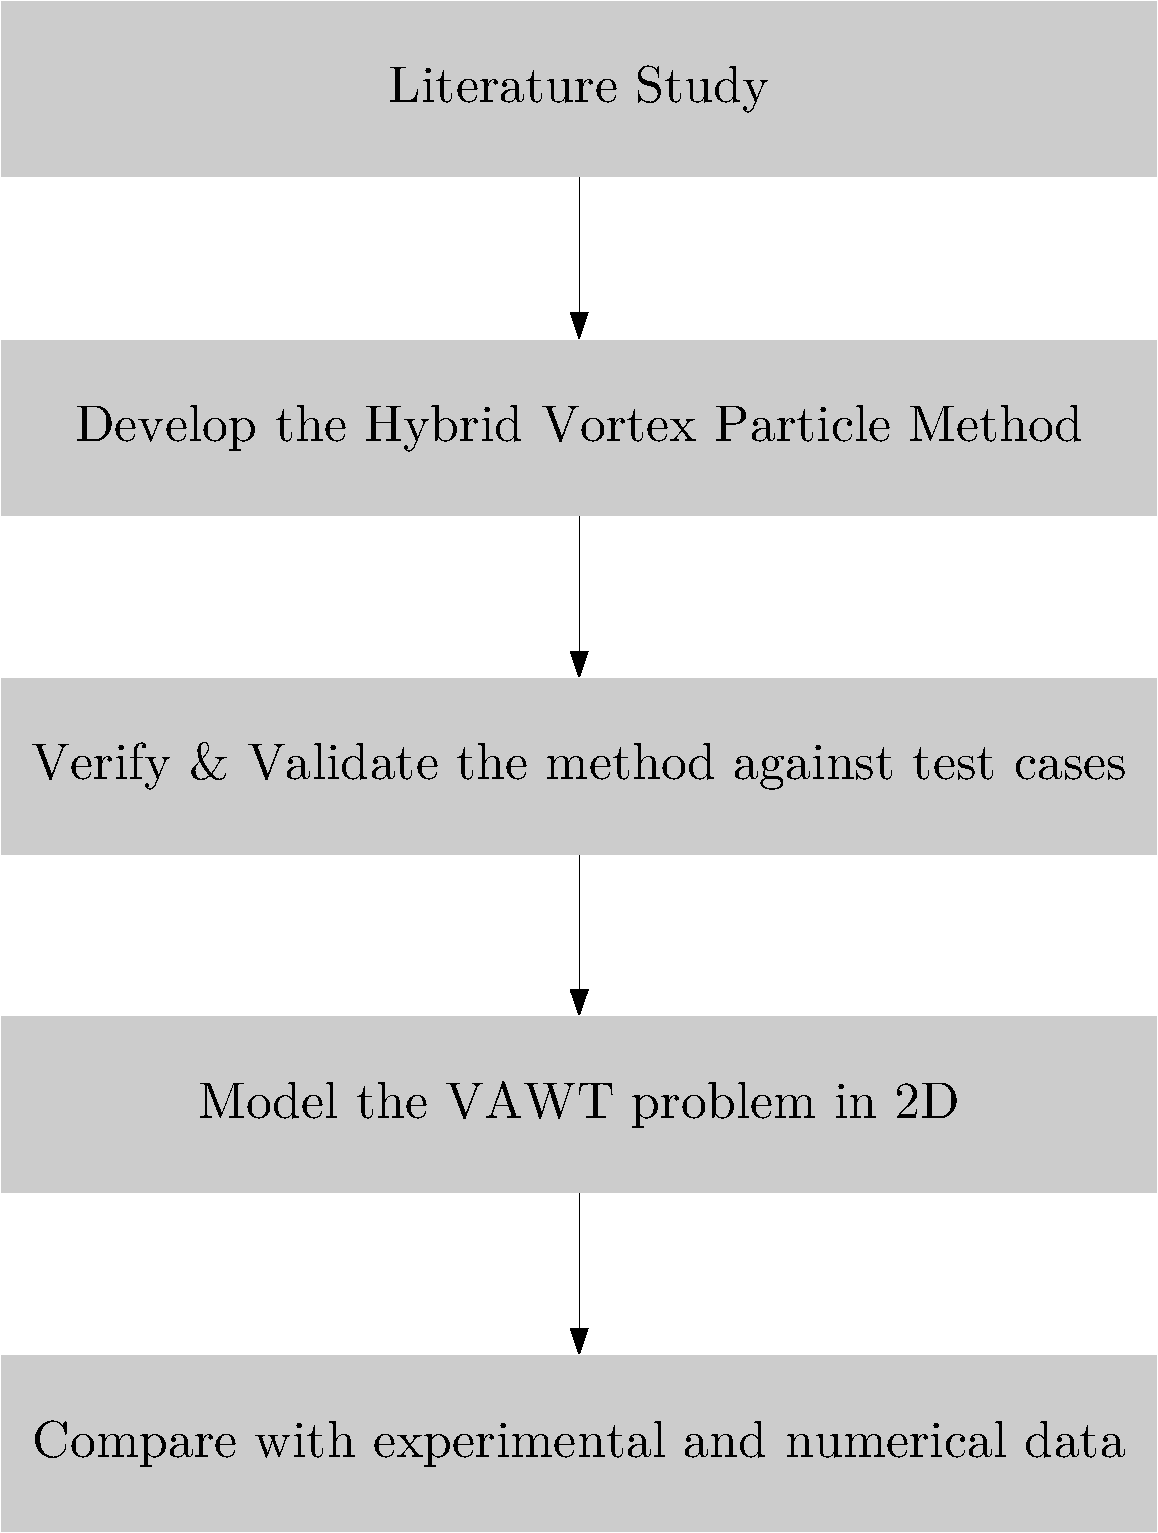
\includegraphics[scale=0.3]{figures/FlowChart.pdf}
\caption{The simplified work breakdown structure of the thesis}
\label{fig:FlowChart}
\end{figure}

The final phase is initiated by the preparation of the draft report. This report will include the verification and the validation of the work and will be carefully discussed with the supervisors. Once the green light if given, the project will be concluded with the request for examination data, submitting the documents and preparation for the graduate presentation. A detailed schematic of the thesis work can be investigated in the gantt chart \ref{fig:GanttChart}.\\

\begin{figure}[p]
\centering
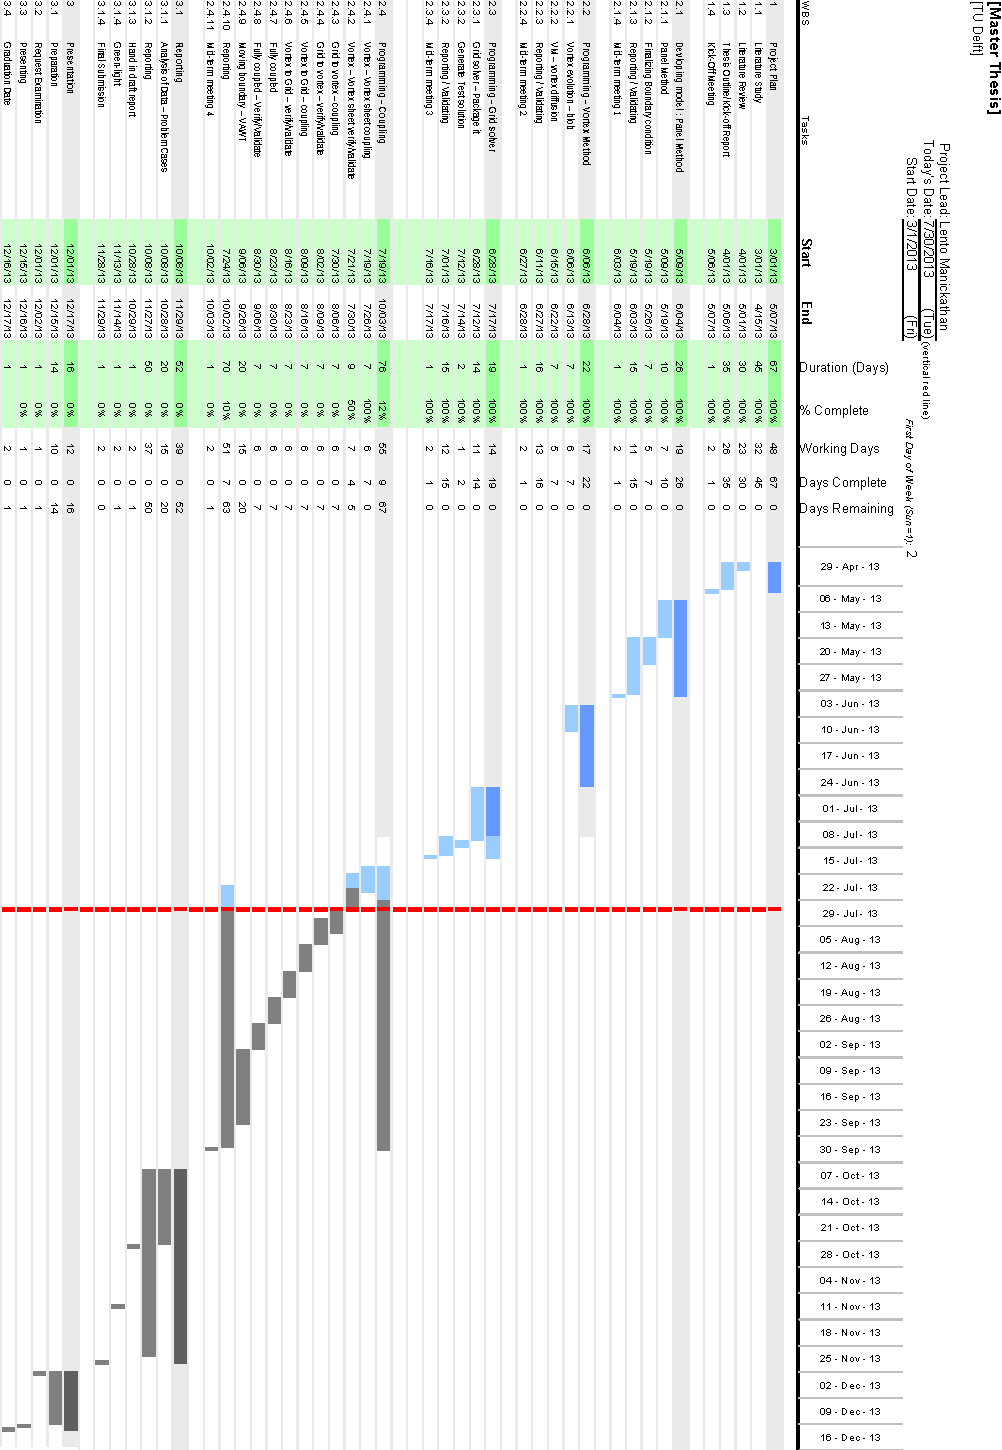
\includegraphics[scale=0.75]{figures/GanttChart.pdf}
\caption{Detailed Gantt chart of the thesis}
\label{fig:GanttChart}
\end{figure}

\newpage

\section{Summary of Project}
%\label{sec:conclusions}

%The conclusions regarding what you are proposing should be written in a precise, unique, clear and accurate manner. Always check if they are well supported by the work you presented in the paper and check them against the main literature so that you can make a statement about the longer-term impact of your work on the body of knowledge? Lift the most important conclusions into the Executive Summary and check that both are consistent, also with the Introduction as the Executive Summary, Introduction and Conclusion form the key points of entry and exit into the work and make a big impact on accessibility and getting across the relevance!

In conclusion, this thesis will be focused on developing an efficient and accurate numerical method to simulate the complex flow phenomenons of a Vertical-Axis Wind Turbine.\\

During the initial stages, a strong theoretical basis will be established before reaching the main development process. During this stage, the innovativeness of the method will be established. The main work will the development of the tool, its verification and the validation against the test cases: dipole-wall interaction, impulsively starting cylinder, multiple geometries, and finally simulating the moving geometry. Concise mid-term reports will be handed once the validation of each of the components is done so that a detailed conversation can me maintained with the supervisor and if possible publishing the results. Before reaching the final stages, the draft report will be made to have ensure smooth transition to the graduation.\\

%\newpage
%
%\bibliographystyle{plain}
%\bibliography{../library}

%List all references consistently, using one of the preferred approaches. The key thing is that the referred to author is given credit through their earlier work, that this is dated to show the chronological order of developments, and that the reader has enough information to go and find that specific reference. Relative to the latter point: where was the conference and did the proceedings have an ISBN number; or if a book what is the ISBN number and publisher, or if a journal paper what was the volume or edition number and certainly page number. The strongest references are ones that have been reviewed prior to publication (journals for example) and the weakest are web sites and popular publications. Only reputable websites (from a society or major industry player) should be included and the date of access should be noted. If at all possible stay away from web references as they are so uncontrolled as sources of information.

%\LaTeX {} template based on \cite{template}.

%\end{document}